\documentclass[10pt]{scrreprt}
\usepackage[utf8]{inputenc}
\usepackage{amsfonts}
\usepackage{amsmath}
\usepackage{amssymb}
\usepackage{commath}
\usepackage[ngerman]{babel}
\usepackage{enumitem}
\usepackage{booktabs}
\usepackage{longtable}
\usepackage{relsize}
\usepackage{pgfplots}
\usepackage{csvsimple}
\usepackage{pgfplotstable}
\usepackage{siunitx}
\usepackage{fancyhdr}
\usepackage{color}
\usepackage{float}
\usepackage{listings}

\definecolor{mygreen}{RGB}{28,172,0} % color values Red, Green, Blue
\definecolor{mylilas}{RGB}{170,55,241}


\lstset{language=Matlab,%
%basicstyle=\color{red},
breaklines=true,%
morekeywords={matlab2tikz},
keywordstyle=\color{blue},%
morekeywords=[2]{1}, keywordstyle=[2]{\color{black}},
identifierstyle=\color{black},%
stringstyle=\color{mylilas},
commentstyle=\color{mygreen},%
showstringspaces=false,%without this there will be a symbol in the places where there is a space
%numbers=left,%
%numberstyle={\tiny \color{black}},% size of the numbers
%numbersep=9pt, % this defines how far the numbers are from the text
emph=[1]{for,end,break},emphstyle=[1]\color{red}, %some words to emphasise
%emph=[2]{word1,word2}, emphstyle=[2]{style},
}

\setlength\parindent{0pt}

\setcounter{chapter}{5}
\setcounter{secnumdepth}{3}
\setcounter{figure}{12}


\pagestyle{fancy}
\fancyhf{}
\lhead{GPET Versuch 6}
\rhead{Tim Luchterhand, Paul Nykiel}
\cfoot{\thepage}

\author{Tim Luchterhand, Paul Nykiel \protect\\ tim.luchterhand@uni-ulm.de, paul.nykiel@uni-ulm.de}
\title{GPET Versuch 6 --- Karl Willy Wagner Versuch}
\subtitle{Gruppe: Dienstag14}

\begin{document}
    \maketitle
    \section{Bestimmung der Grenzfrequenz}
    \paragraph{Aufgabe}
    Bestimmen Sie die Grenzfrequenz eines RC-Tiefpasses ($R = 1\si{k\ohm}$ und $C = 2.2\si{\mu\farad}$) mit
    Hilfe des Oszilloskops. Berechnen Sie damit und mit der Formel aus Gl. 13 den Innenwiderstand des Oszilloskops.
    \begin{enumerate}
        \item Messen Sie mit dem Multimeter die exakten Werte $R$ und $C$ der Bauteile.
        \item Bauen Sie die Schaltung auf und messen Sie mit Hilfe des Oszilloskops die Grenzfrequenz
                $f_g$. Gehen Sie möglichst sorgfältig vor.
        \item Geben Sie eine geeignete Formel zur Bestimmung des Innenwiderstands des Oszilloskops an.
        \item Bestimmen Sie den Innenwiderstand für die gemessene Frequenz bei einem Messfehler
                (der Grenzfrequenz) von $\pm1\%$. Also $R_{i,f_g}$, $R_{i,f_g+1\%}$ und $R_{i,f_g-1\%}$.
        \item Bestimmen Sie den Innenwiderstand $R_i$ des Oszilloskops mit Hilfe des Multimeters.
        \item Wie groß ist der Innenwiderstand $R_i$ laut Beschreibung des Oszilloskops?
        \item Geben Sie ein kurzes Fazit für diesen Teil des Versuchs.
    \end{enumerate}

    \paragraph{Protokoll}
    %TODO Vorbereitung: Innenwiderstand Oszi, Formel
    \begin{enumerate}
        \item Mit Multimeter gemessene Werte:
            \begin{eqnarray*}
                R &=& 997\si{\ohm}\\
                C &=& 2.23\si{\mu\farad}
            \end{eqnarray*}

            Die gemessenen Werte weichen um weniger als $2\%$ von den angegebenen
            Bauteilwerten ab.
        \item
        Vorgehensweise:

        Auf dem Oszilloskop werden die Ein-~und Ausgangsspannungen dargestellt und
        mit der Measure-Funktion jeweils die Spitze-Spitze-Spannung bestimmt.
        Dann wir die Frequenz der Eingangsspannung so lange verändert, bis
        $\abs{\underline{U_2}} \approx 0.7 \cdot \abs{\underline{U_1}}$ gilt (siehe
        Screenshot).

        Bestimmte Grenzfrequenz:

        \begin{equation*}
            f_g \approx 76\si{\hertz} \pm 2\si{\hertz}
        \end{equation*}

        \begin{center}
            \begin{figure}[H]
                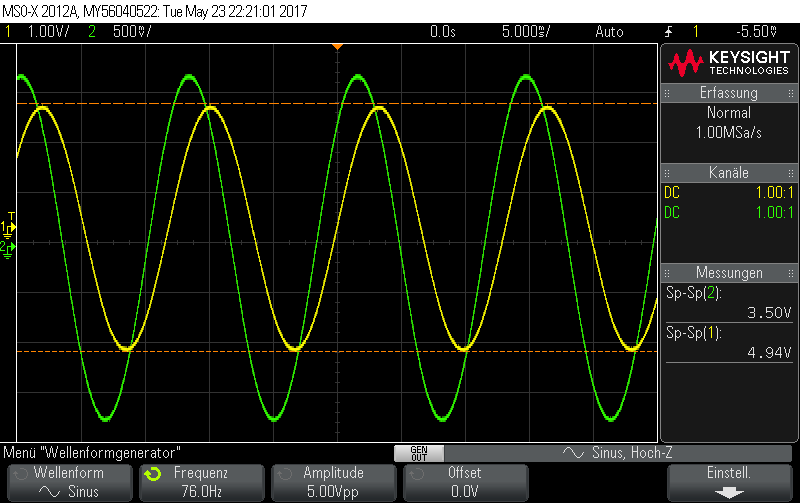
\includegraphics[width=\textwidth]{scope_4.png}
                \caption{Bestimmung der Grenzfrequenz}
            \end{figure}
        \end{center}

        \item
            Der RC-Tiefpass ist durch den Innenwiderstand des Oszilloskops
            belastet, das heißt: $R_L = R_{innen}$. Daraus folgt:
            \begin{eqnarray*}
                A &=& \frac{1}{\sqrt{{\left(1+\frac{R}{R_L}\right)}^2 + {(\omega R C)}^2}}\\
                \Leftrightarrow
                R_i &=& R_L = \frac{R}{\sqrt{\dfrac{1}{A^2} -{(\omega R C)}^2} - 1}
            \end{eqnarray*}
        \item
            \begin{eqnarray*}
                R_{i,f_g} &=& -1067\si{\ohm}\\
                R_{i,f_g+1\%} &=& -1081\si{\ohm}\\
                R_{i,f_g-1\%} &=& -1041\si{\ohm}\\
            \end{eqnarray*}
            Offensichtlich können negative Widerstandswerte nicht sein.
        \item
            Mit Multimeter gemessener Innenwiderstand:
            \begin{equation*}
                R_i = 1.00\si{M\ohm}
            \end{equation*}
        \item
            Innenwiderstand laut Beschreibung:
            \begin{equation*}
                R_i = 1 \si{M\ohm} \pm 2\%
            \end{equation*}
        \item \textbf{Fazit:}
            Wie an den Ergebnissen zu erkennen ist, eignet sich dieses Verfahren
            nicht zur Bestimmung von Innenwiderständen. Theoretisch sollte die
            Vorgehensweise sinnvolle Ergebnisse liefern, da diese aber stark von
            der bestimmten Grenzfrequenz abhängen, können schon sehr kleine
            Ungenauigkeiten von weniger als $1\%$ die komplette Messung unbrauchbar
            machen. Ein perfektes Beispiel dafür sind unsere Messergebnisse, die
            trotz korrekter Rechnung und mehrfacher Messung physikalisch schlicht
            und einfach keinen Sinn machen.
    \end{enumerate}

    \section{Zeitverhalten eines Hochpasses}
    \paragraph{Aufgabe}
    \begin{center}
        \begin{figure}[H]
            
\includegraphics[width=\textwidth]{abb8.png}
            \caption{Hochpass erster Ordnung}
            \label{fig:abb8}
        \end{figure}
    \end{center}
    Messen Sie die Abfallzeit der Schaltung aus~\ref{fig:abb8} für folgende Bauteil- und
    Spannungswerte:
    \begin{eqnarray*}
        R &=& 100\si{\ohm}\\
        C &=& 2.2\si{\mu \farad}\\
            \underline{U_1} &=&
            \begin{cases}
                t < 0& -2.5\si{\volt}\\
                t \geq 0& 2.5\si{\volt}
            \end{cases}
    \end{eqnarray*}
    \begin{enumerate}
        \item Bauen Sie das Filter aus~\ref{fig:abb8} auf und messen Sie die Abfallzeit einmal von Hand
            und einmal mit Hilfe der eingebauten Rise-/Falltime Messung.
        \item Berechnen Sie den theoretisch zu erwartenden Wert.
    \end{enumerate}

    \paragraph{Protokoll}
    %TODO Formel
    \begin{center}
        \begin{figure}[H]
            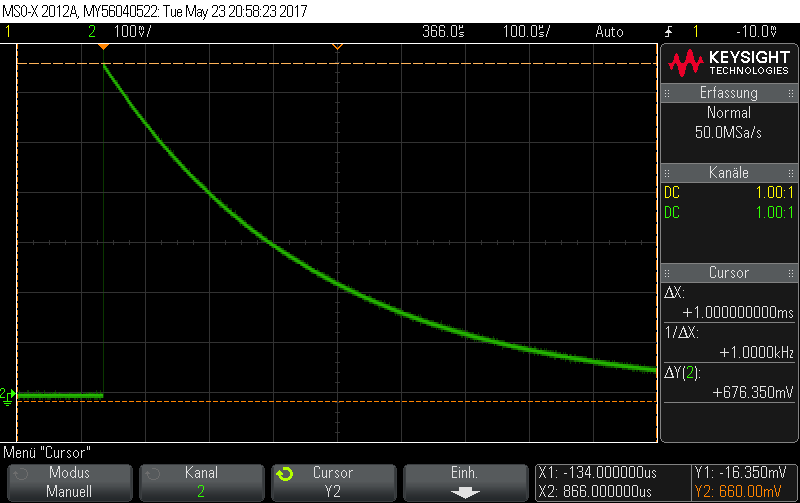
\includegraphics[width=\textwidth]{scope_1.png}
            \caption{Messung des Maximalwerts mit Cursor}
        \end{figure}
    \end{center}
    \begin{center}
        \begin{figure}[H]
            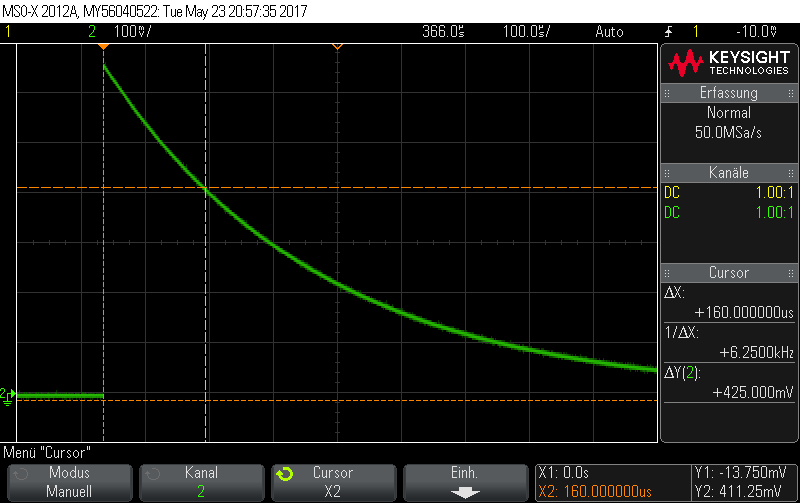
\includegraphics[width=\textwidth]{scope_0.png}
            \caption{Messung von $\tau$ mit Cursor}
        \end{figure}
    \end{center}

    \begin{center}
        \begin{figure}[H]
            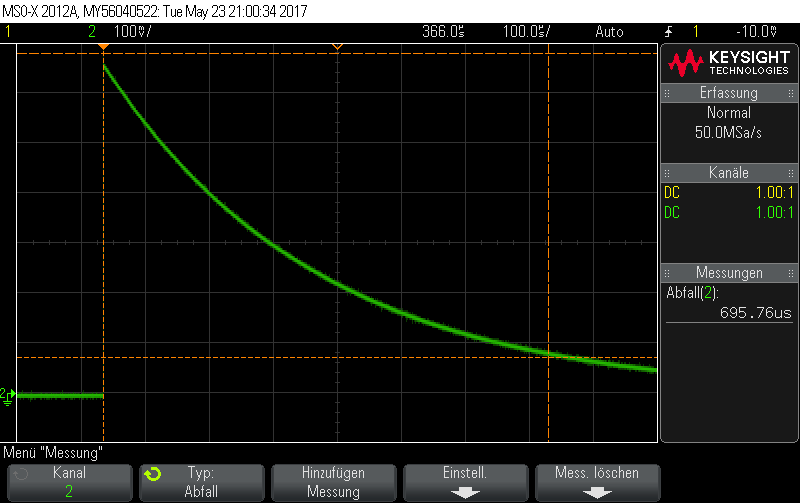
\includegraphics[width=\textwidth]{scope_2.png}
            \caption{Messung der Anstiegszeit mit Measure}
        \end{figure}
    \end{center}


    Bei der Messung mit Cursor wurde aus genauigkeitsgründen $\tau$ bestimmt,
    da man für die Anstiegszeit $t_a$ sonst $3$ Werte bestimmen muss, was zu
    höheren Messungenauigkeiten führt. $t_a$ lässt sich dann wie folgt bestimmen:
    \begin{eqnarray*}
        \tau_{cursor} &=& 160 \si{\mu\second}\\
        {t_a}_{cursor} &\approx& 2.2 \tau_{cursor} = 351 \si{\mu\second}\\
        {t_a}_{measure} &=& 695.76 \si{\mu\second}\\
        {t_a}_{theoretisch} &\approx& 2.2\tau = 2.2 \cdot RC = 483 \si{\mu\second}
    \end{eqnarray*}

    Man erkennt, dass der theoretische Wert zwischen beiden Messwerten liegt.
    Interessant ist, dass der manuell bestimmte Wert näher am theoretischen liegt,
    als der automatisch bestimmte. Bei der Messung mit measure ist aufgefallen,
    dass sich die automatisch bestimmten Messpunkte ständig verändert haben, was
    dann auch Änderungen von über $100\si{\mu\second}$ verursachte. Die Mesungenauigkeiten
    bei der manuellen Messung lassen sich auf einen systematischen Fehler zurückführen.

    \section{Bandpass}
    \paragraph{Aufgabe}
    \begin{center}
        \begin{figure}[H]
            
\includegraphics[width=\textwidth]{abb17.png}
            \caption{Unbelasteter Bandpass erster Ordnung}
            \label{fig:abb17}
        \end{figure}
    \end{center}
    Im Folgenden soll das Übertragungsverhalten eines Bandpasses 1. Ordnung untersucht
    werden. Bauen Sie dazu das Bandpass-Filter aus~\ref{fig:abb17} mit $R = 100 \si{\ohm}$ und $C = 2.2 \si{\mu\farad}$
    auf. Als Induktivität verwenden Sie eine Spule mit 250 Windungen.
    Nehmen Sie die Übertragungsfunktion mit Hilfe der Matlab-GUI (100 Punkte, $1\si{\volt}_{pp}$,
    $100\si{\hertz}$–$100\si{k\hertz}$, log) auf und fügen Sie das Diagramm in Ihr Protokoll ein. Diskutieren
    Sie Ihre Ergebnisse.

    \paragraph{Protokoll}
    \begin{center}
        \begin{figure}[H]
            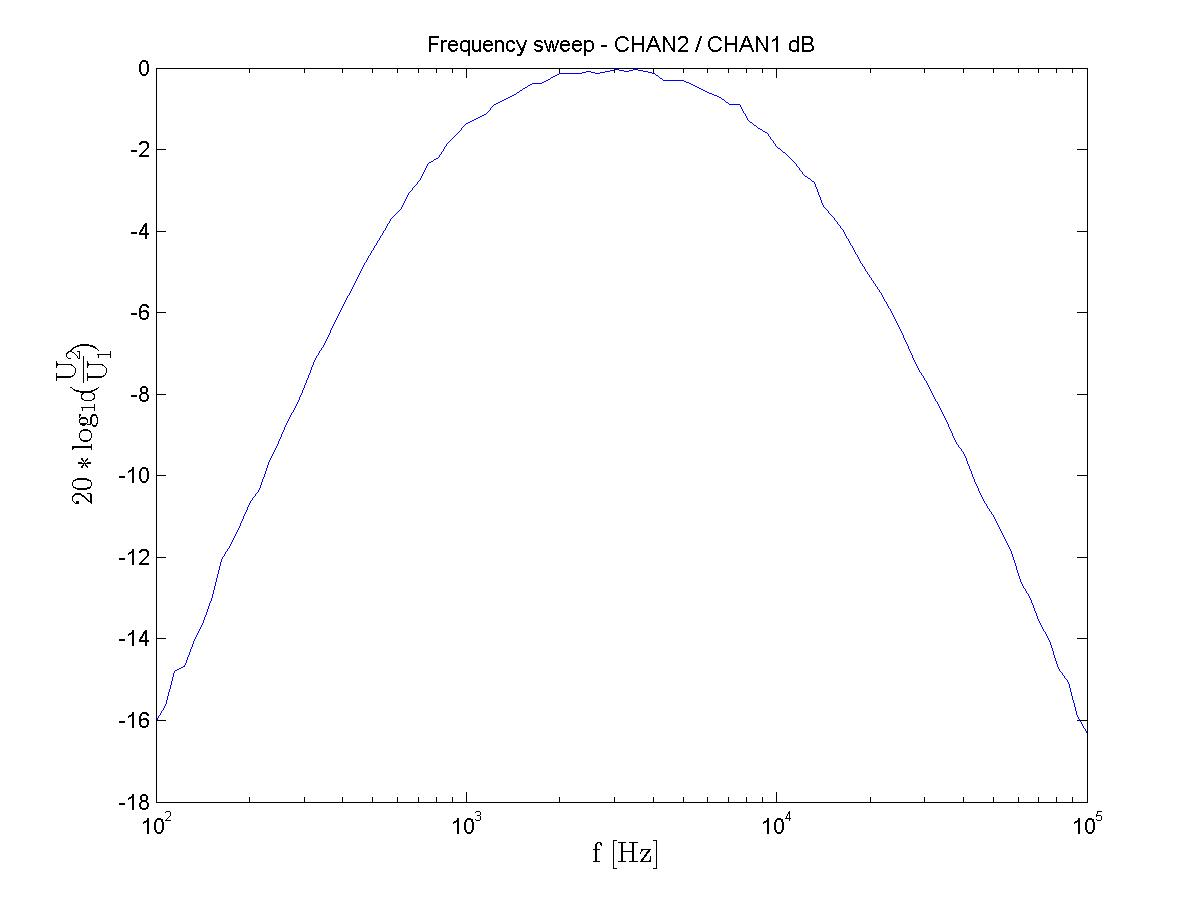
\includegraphics[width=\textwidth]{FS_53_frequencysweep_ylogxlog.jpg}
            \caption{Übertragungsfunktion des Bandpass}
            %\label{fig:abb19}
        \end{figure}
    \end{center}
    Man erkennt, dass die Übertragungsfunktion zu den Extremwerten hin jeweils
    gegen $-\infty$ abfällt und nur in der Mitte (in logarithmischer Darstellung)
    des gemessenen Frequenzbandes  gegen 0 geht. Das bedeutet also, dass nur ein
    bestimmtes Frequenzband ungedämpft bleibt (zwischen $10^3\si{\hertz}$ und
    $10^4\si{\hertz}$). Eine solche Charakteristik ist typisch für einen Bandpassfilter

    \section{Bandsperre}
    \paragraph{Aufgabe}
    \begin{center}
        \begin{figure}[H]
            
\includegraphics[width=\textwidth]{abb19.png}
            \caption{Unbelastete Bandsperre erster Ordnung}
            \label{fig:abb19}
        \end{figure}
    \end{center}
    Weiter soll das Übertragungsverhalten einer Bandsperre 1.Ordnung untersucht werden.
    Bauen Sie dazu die Bandsperre aus~\ref{fig:abb19} mit $R = 100 \si{\ohm}$ und $C = 2.2 \si{\mu\farad}$ auf. Als
    Induktivität verwenden Sie eine Spule mit 250 Windungen.
    Nehmen Sie die Übertragungsfunktion mit Hilfe der Matlab-GUI (100 Punkte, $1\si{\volt}_{pp}$
    $100\si{\hertz}$–$100\si{k\hertz}$, log) auf und fügen Sie das Diagramm in Ihr Protokoll ein. Diskutieren
    Sie Ihre Ergebnisse.
    \paragraph{Protokoll}
    \begin{center}
        \begin{figure}[H]
            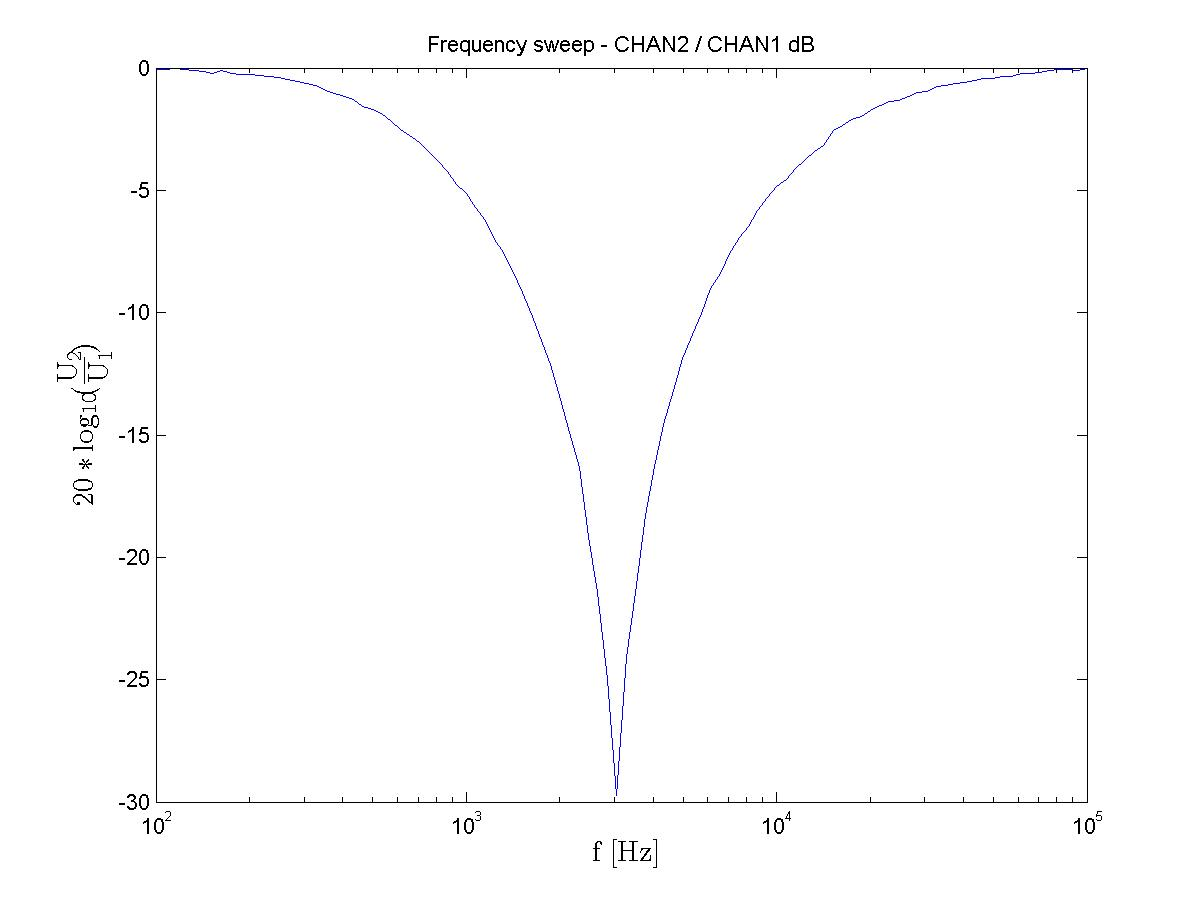
\includegraphics[width=\textwidth]{FS_54_frequencysweep_ylogxlog.jpg}
            \caption{Übertragungsfunktion der Bandsperre}
            %\label{fig:abb19}
        \end{figure}
    \end{center}
    Man erkennt, dass die Übertragungsfunktion zu den Extremwerten hin jeweils
    gegen 0 und nur in der Mitte (in logarithmischer Darstellung)
    des gemessenen Frequenzbandes  gegen $-\infty$ geht. Das bedeutet also, dass
    ein bestimmtes Frequenzband herausgefiltert wird (zwischen $10^3\si{\hertz}$
    und $10^4\si{\hertz}$). Eine solche Charakteristik ist typisch für eine
    Bandsperre.


    \section{Frequenzbereich und Audio-Filterung}
    \paragraph{Aufgabe}
    \begin{enumerate}
        \item Hören Sie sich zunächst das Audio-Sprach-Signal an. In welchem Frequenzbereich
            befindet sich die Störung?
        \item Realisieren Sie mit zwei Kondensatoren ($C = 2.2 \si{\mu\farad}$) und einer Spule (500 Windungen)
            ein Hochpass-Filter in T-Schaltung und zeigen Sie den Aufbau Ihrem Tutor.
        \item Bestimmen Sie den ohmschen Widerstand des Kopfhörers.
        \item Messen Sie die Übertragungsfunktion des Hochpass-Filter einmal ohne und einmal
            mit angeschlossener Last (Kopfhörer) und stellen Sie diese in zwei Diagrammen
            dar (200 Punkte, $100\si{\hertz}$–$100\si{k\hertz}$, log.). Verwenden Sie dazu die Matlab-GUI
            ($500\si{m\volt}_{pp}$). Speichern Sie die Plots und fügen Sie diese in Ihr Protokoll ein. Erklären
            Sie die Verläufe der Funktionen für kleine und große Frequenzen.
        \item Hören Sie sich einmal das ungefilterte und einmal das gefilterte Audio-Sprach-Signal
            an. Welche Person spricht da und welchen Satz sagt sie am Ende?
    \end{enumerate}

    \paragraph{Protokoll}
    \begin{enumerate}
        \item Das Audiosignal wir überdeckt von einem tiefen Summen. Die Frequenz
        des Störsignals liegt also schätzungsweise zwischen $20\si{\hertz}$ und
        $500\si{\hertz}$.
        \item
            Innenwiderstand des Kopfhörers bestimmt mit Multimeter:
            \begin{equation*}
                R_i = 37\si{\ohm} \pm 20\si{\ohm}
            \end{equation*}
            Bemerkung:

            Aufgrund der mangelhaften Qualität des Kopfhörers und der Kabel, ergaben
            sich absolute Messungenauigkeiten von bis zu $20\si{\ohm}$.
        \item
            \begin{center}
                \begin{figure}[H]
                    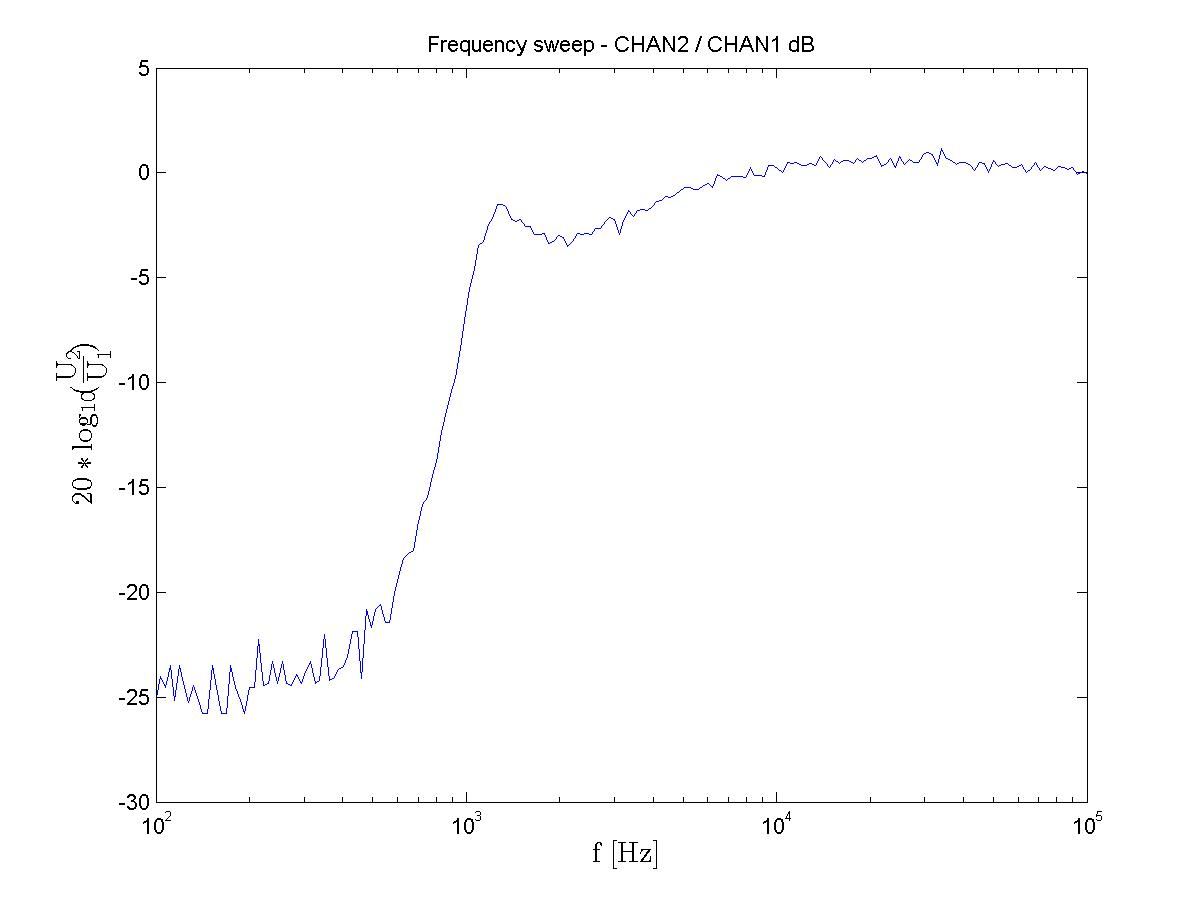
\includegraphics[width=\textwidth]{FS_55M_frequencysweep_ylogxlog.jpg}
                    \caption{Übertragungsfunktion des Hochpass mit Last}
                    \label{fig:abbM}
                \end{figure}
            \end{center}
            \begin{center}
                \begin{figure}[H]
                    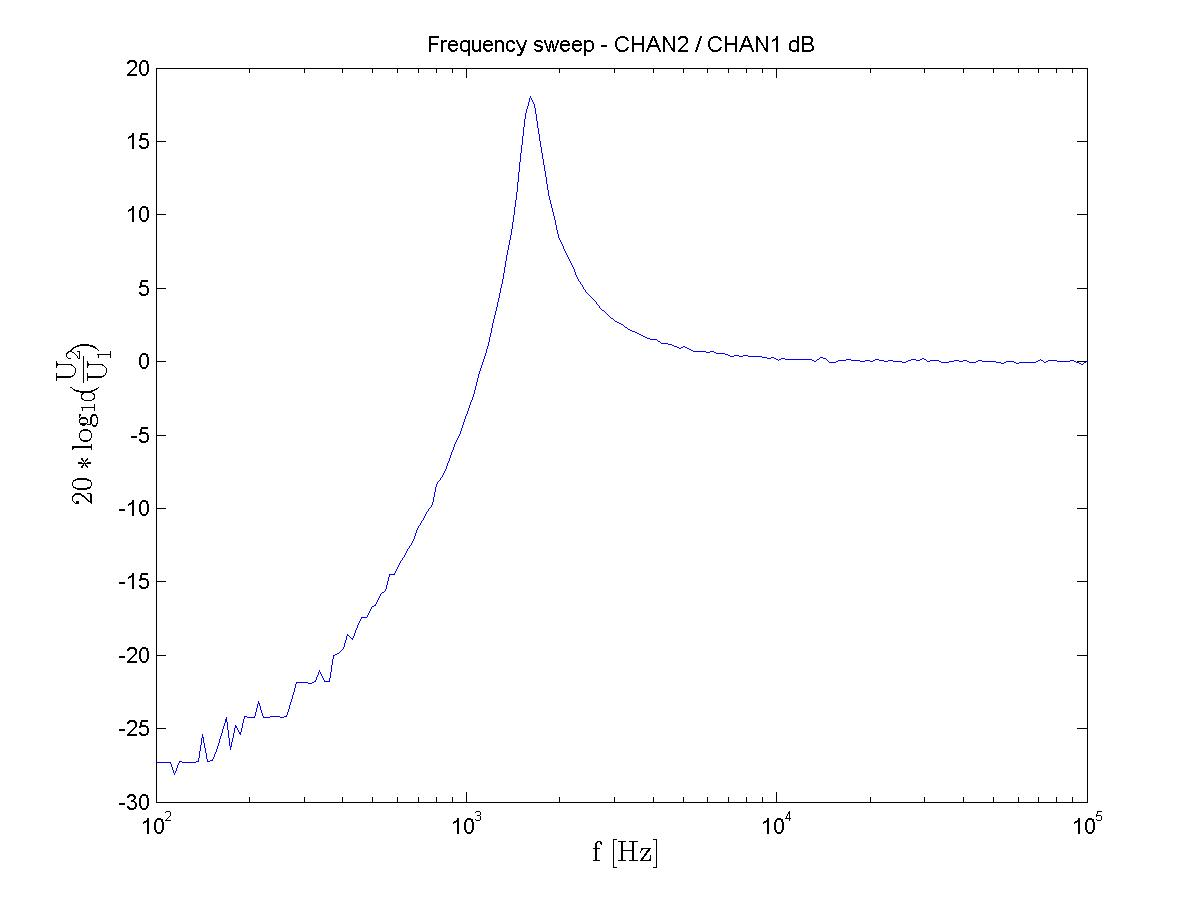
\includegraphics[width=\textwidth]{FS_55O_frequencysweep_ylogxlog.jpg}
                    \caption{Übertragungsfunktion des Hochpass ohne Last}
                    \label{fig:abbO}
                \end{figure}
            \end{center}

            Beide Verläufe zeigen die typischen Eigenschaften der Übertragungsfunktion
            eines Hochpassfilters: Für kleine Frequenzen geht diese gegen $-\infty$
            und für große Frequenzen gegen 0. In beiden Abbildungen ist außerdem
            ein Peak bei der Grenzfrequenz zu erkennen. In Abb.~\ref{fig:abbO}
            geht dieser Peak sogar weit über 0dB hinaus (bis ca. 18dB). Dies lässt
            sich folgendermaßen erklären:

            Der Hochpass aus Spule und Kondensator verhält sich zusätzlich wie
            ein LC-Schwinkreis, der bei der Grenzfrequenz seine Resonanzfrequenz
            besitzt. Bei dieser Frequenz findet also ein Überschwingen statt, da
            am Ausgang mehr Spannung anliegt, als am Eingang. In Abb.~\ref{fig:abbM}
            ist dieser Peak deutlich schwächer und reicht nicht über die 0dB hinaus.
            Das ist durch die zusätzliche Dämpfung durch die Innenimpedanz des
            Kopfhörers zu erklären. Diese Impedanz ist außerdem für die Verschiebung
            der Grenzfrequenz in Abb.~\ref{fig:abbM} verantwortlich.

            Zu guter Letzt ist in Abb.~\ref{fig:abbM} vermehrt Rauschen zu erkennen,
            was einerseits durch die Indutivität des Kopfhörers, aber hauptsächlich
            durch die schlechten Kopfhörerkabel verursacht wird.


        \item
            Im Vergleich zum Originalsignal lässt sich die Stimme deutlich besser
            erkennen. Auch wenn es nicht möglich war, den Sprecher oder das Gesprochene
            zu identifiziern, so konnte man trotzdem die gesprochene Sprache als
            Englisch einordnen.
    \end{enumerate}
\end{document}
